
In Section \commentBN{insert section} we examined different functions we can use to aggregate preferences and select a common choice. As we saw, different functions lead to different outcomes and, starting from the same preference profile we can select different winners depending on the voting rule used. Consider an everyday scenario as example: movies ratings. 

Reviews have always been important bases for many in their daily choices, from restaurants critiques to theaters opening-night reviews. With the growth of technological progress and increasingly accessible communication platforms, reviews soon expanded not only to professional critics but to anyone. Today, anyone with internet access can express their opinions about everything and it is increasingly rare to watch a movie, book a restaurant or buy a vacuum cleaner without reading other people's opinions about it. Consider the movie example. Rotten Tomatoes, IMDb and Metacritic are only few examples of review-aggregation websites for movies, television and games. The best film of all times according to IMDb is \textit{"The Shawshank Redemption"}, but this does not appear not even among the best 100 movies according to Rotten Tomatoes and Metacritic. The reason is because these platform all use a different aggregation method. \Cref{tab:movies} and \Cref{fig:movies} show two movies examples. 

%"Avengers: Endgame" (2019) 
%Rotten Tomatoes 94$\%$  (8.20 out of 10 average rating)
%IMDB 8.4 Arithmetic mean = 8.4   Median = 9
%Metacritic 78/100

\begin{table}[h]
	\label{tab:movies}
	\tiny{
	\begin{tabular}{cccc}
		& Rotten Tomatoes & IMDB & Metacritic \\
		La tigre e la neve & 20$\%$ 4.00 out of 10 average rating  (84$\%$ audience) & 7.1 Arithmetic mean = 7,3   Median = 7 & Metracritic 22/100 (User Score 7.9, Arithmetic mean = 25.8) \\
		Ghostbusters & 74$\%$ 6.50 out of 10 average rating  audience 49$\%$ & 6.5  Arithmetic mean = 5,3   Median = 6 & 60/100 (User Score 2.8, Arithmetic mean = 25.8)
	\end{tabular}
}
\end{table}


%"" 
%Rotten Tomatoes 20$\%$ 4.00 out of 10 average rating  (84$\%$ audience)
%IMDB 7.1 Arithmetic mean = 7,3   Median = 7
%Metracritic 22/100 (User Score 7.9, Arithmetic mean = 25.8)
%
%"Ghostbusters" 2016
%Rotten Tomatoes 74$\%$ 6.50 out of 10 average rating  audience 49$\%$
%IMDB 6.5  Arithmetic mean = 5,3   Median = 6
%Metracritic 60/100 (User Score 2.8, Arithmetic mean = 25.8)

\begin{figure}
	\label{fig:movies}
	\centering
	\begin{subfigure}[b]{1\textwidth}
		\centering
		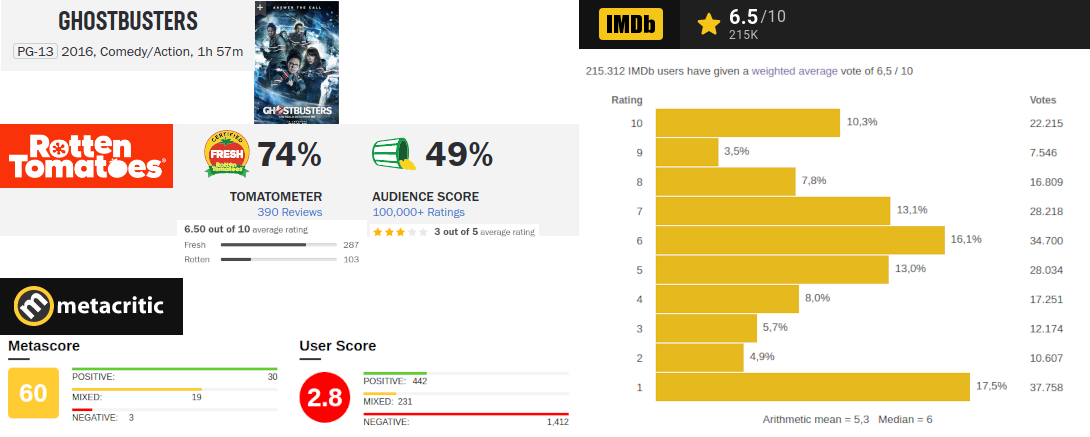
\includegraphics[scale=0.3]{img/ghost.png}
		\caption{}
	\end{subfigure}
	\begin{subfigure}[b]{1\textwidth}
		\centering
		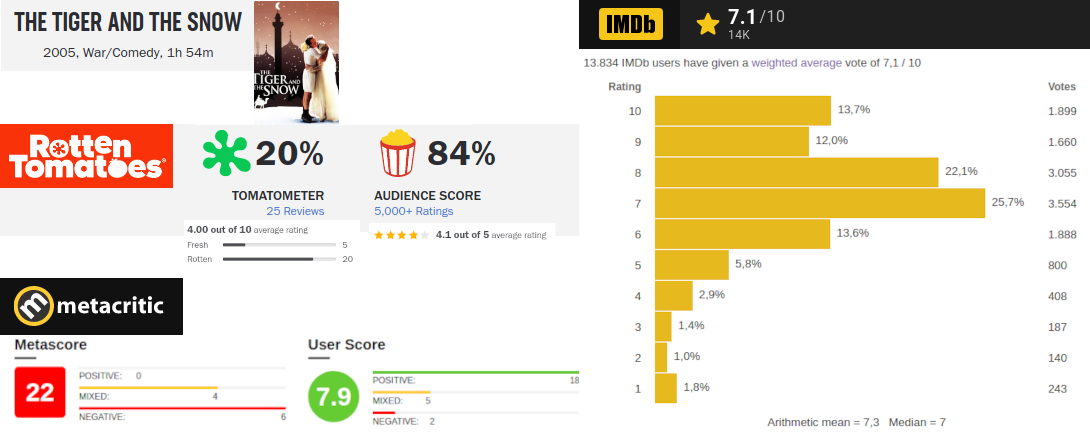
\includegraphics[scale=0.3]{img/tigre.png}
		\caption{}
	\end{subfigure}
	\caption{Ratings from different review-aggregation websites (Rotten Tomatoes, Metacritic and IMDb) for the movies Ghostbusters (a) and The tiger and the snow (b).}
\end{figure}
